%!TEX root = ../assignment1.tex

\section{Findings of Phase 1}

\subsection{Overview Of Data}
In our selection of literature, 6 articles are employed. \citetitle{1} and \citetitle{2} are on project management. \citetitle{3} argues about change management while \citetitle{4} and \citetitle{5} are on risk management. \citetitle{6} gives an overview and an update of information system success and failure, which is composed by an affiliation of famous scholars in the field.

\subsection{Gaps and Solutions}

The gaps and the solutions often express the same meanings but with different wording. Gaps are often stated as "lack of something" while the solutions suggest to supplement the missing part. Therefore, we only collect the proposals that the literature suggests, for the sake of conciseness.

We have extracted 32 sections containing 48 proposals contributing to success, failure or risks from the 6 articles. We have also tagged the affected phases and the affected roles for each proposal. The weights of priority are also recorded and normalized in the researches where the authors conclude with a math model. A baseline value of $1$ is given to those proposals from which the authors have not built a math model.

Using the aforementioned primary themes, regarding the 4 main themes, that is control, process, people and structure here, we have got many findings below:

\subsubsection{Samples: Control}

On page 9 of \citetitle{3}, \citeauthor{3} argue that the design must be established consistently. Obviously, to prevent unnecessary reconfiguration at each implementation stage, a consistent well-thought-out ERP design that meets the needs of the organization should be established.

On page 11 of \citetitle{2}, \citeauthor{2} put emphasis on the suggestion that proactively assesses the performance of a vendor and develop a list of performance metrics for vendors. The project manager should set up objective and clear evaluation criteria for the supplier in advance and ensure that the supplier complies with the evaluation criteria during the implementation of the project. In addition, the project manager should regularly evaluate the progress of the project rather than just evaluating it at the end of the project. Only in this way, once the deviation from the standard occurs, the project manager can know what and why the deviation occurs in time, and take appropriate measures to ensure that the deviation is solved in time. After all, it is not enough to rely solely on the vendor to solve problems themselves. In general, periodically assessment is important because it is a reliable method to help the project manager understanding the situation of that time. Additionally, it is also good to maintain a good vendor-client partnership.

\subsubsection{Samples: Process}
\citeauthor{2} suggests that keep 85\% of business process common and set up a decision committee on page 11 of \citetitle{2}. Better relationship between project managers and the management is pretty important to IT Projects. To establish and maintain a good relationship between them, on the one hand, project manages should keep the project scope as consistent as possible with the management; on the other hand, in order to reduce or avoid the resistance of end users from different regions, product managers should consider forming a priority committee. It can be an important scope management tool because its members come from different regions, so the scope decision process is largely transparent to them.

\citeauthor{6} recommend that it is better to identify the problem before proposing a solution and to understand user requirements before designing a system on page 10 of \citetitle{6}. A common mistake is to start designing a solution only with a rough understanding of the problem to be solved, especially for those experienced people. As the saying goes, a good question is better than a great answer. It can be an essential rule that taking more time to understand the problem before making a decision. (Bergman et al. 2002)

\subsubsection{Samples: People}
In \citetitle{3}, the author argues that it is important to have effective communication at each level. Efficient and effective communication is an integral part of the successful implementation of IT projects. During an IT project life cycle, communication is necessary at every level of the project. According to Mandal and Gunasekaran (2003), opinions from users about their requests, responses, objections or approvals are always important. Project progress should be communicated regularly to management so they can understand the current status of the project. As for the objectives, activities, news or updates, it should be promptly notified to the relevant staff in the project.


To manage the communication process and create a forum is the suggestion given by \citeauthor{2} when talking about success of building an ERP system. Therefore, the project manager should work hard to manage the communication process, including communicating with management and communicating downwards. Based on this, it is necessary to create a forum where stakeholders can prioritize and discuss issues. There are various conflicts between business and IT projects, and successfully managing these conflicts is essential to the success of IT projects. Guiding end-users to participate in projects can effectively reduce or resolve these conflicts, and those projects that end users actively participate in are often successful.

\subsubsection{Samples: Structure}
\citeauthor{6} believe that getting top management support is important for the successful implementation of IT on page 10 of \citetitle{6}. According to Markus (1983) and Elbanna (2012), getting top management support is still the most important principle for helping project success. It is reasonable since projects usually cannot run smoothly without top management support, especially when the project is under construction.

For vendor support, \citeauthor{6} also suggest that it is important to obtain “independent” advice from a consultant. As for selecting an appropriate vendor, in order to obtain objective and fair comparison results, independent third-party professional consultants should be sought (Pollock and Williams 2009).

\subsection{Evaluation Of Solutions}
\label{section:evaluation}
To clarify the result, we collect the data into a spreadsheet in which contains the following criteria: No., proposal, article identifier, coding identifier, affected phases, affected roles.
% \begin{table}[ht] 
% \caption{Coding(header only)}
% \resizebox{\columnwidth}{!}{%
% \csvautotabular{tables/coding_sample.csv}
% }
% \label{tab:sample}
% \end{table}

With the defined method, we tag our research contexts in the following sequence.
$C_{1}$ is \citetitle{1}.
$C_{2}$ is \citetitle{2}.
$C_{3}$ is \citetitle{3}.
$C_{4}$ is \citetitle{4}.
$C_{5}$ is \citetitle{5}.

According to the defined method, we have everything for the evaluation process. Due to the fact that the studies are not conducted with a math model in $C_{2}$ and $C_{4}$, we assume all the solutions from the aforementioned researches are of equal importance. Therefore, we pad the cross-contextual coefficient with a baseline value of 1 to $\mathit{f_{C_{2,j}}}$ and $\mathit{f_{C_{4,j}}}$.

Using the formula \ref{final}, we calculate the global influence score for each proposal. Here is a visualization of the scores of all the proposals.

\begin{figure}[ht]
\centering
\resizebox{\columnwidth}{!}{%
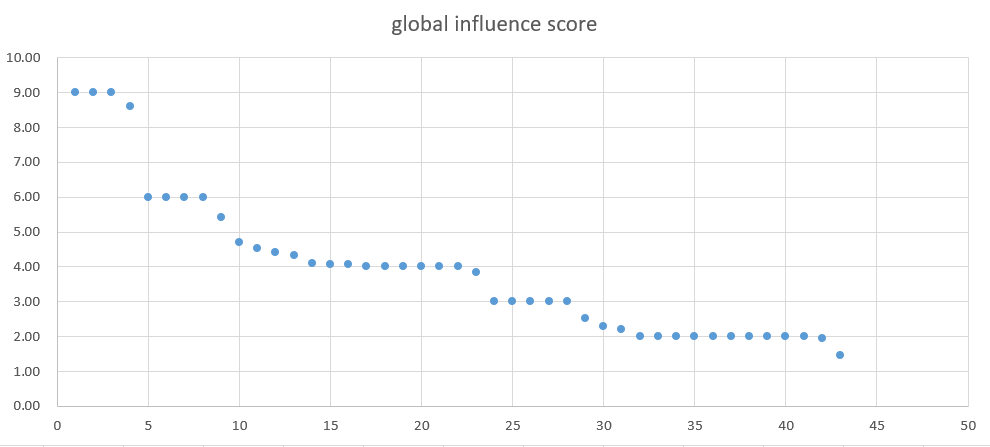
\includegraphics{global_influence_score.png}
}
\end{figure}

In the plot, the horizontal axis stands for all the proposals in context $\mathbb{C}$ and the vertical axis for global influence score. It is clear that there are 4 proposals of significant influence clustering at the top followed by a second group at range roughly between 4 to 6. The trailing group of low influence score occupies the range between 1 to 3.

\subsection{Result Of Evaluation}
For the effectiveness and conciseness, we truncate the trailing group scored lower than average($\bar{g}=3.60$), which is also the trailing group. We obtain the following list of solutions.

\begin{table}[ht]
\caption{Solution List Of Phase 1}
\resizebox{\columnwidth}{!}{%
\csvautotabular{tables/solutions.csv}
}
\label{tab:solution}
\end{table}

% To track their origins of sources, we mark them with the article themes as shown in \ref{tab:solution}. There are 10 solutions about project management, 8 about risk management and 5 about change management.
